\section{SciPy}
\begin{itemize}
	\item Python-Bibliothek
	\item[\-] \texttt{from scipy import integrate, interpolate, optimize, signal, ...}
	\item Basiert auf NumPy
	\item Enthält numerische Algorithmen und mathematische Werkzeuge\\
	\item \url{https://docs.scipy.org/doc/scipy/reference/}
\end{itemize}

\begin{minipage}[t]{0.49\textwidth}
	\subsection{SciPy.Interpolate}
	\begin{itemize}
		\item 1-dimensionale Interpolation
		\item Mehrdimensionale Interpolation
		\item Splines
		\item API-Referenz: \url{https://docs.scipy.org/doc/scipy/reference/interpolate.html}
	\end{itemize}
\end{minipage}
\hspace{0.02\textwidth}
\begin{minipage}[t]{0.49\textwidth}
	\lstinputlisting{listings/v9_interpolate1.py}
	Stützwerte für x und y:
	\lstinputlisting{listings/v9_interpolate2.py}
\end{minipage}\\[12pt]

\begin{minipage}[t]{0.54\textwidth}
	Interpolationsfunktionen erstellen:
	\lstinputlisting{listings/v9_interpolate3.py}
\end{minipage}
\hspace{0.02\textwidth}
\begin{minipage}[t]{0.44\textwidth}
	$\quad$\\[1pt]
	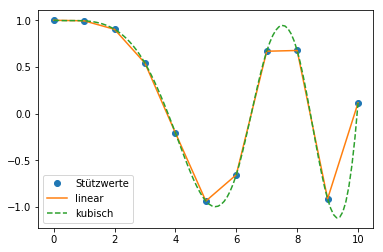
\includegraphics[width=\textwidth]{images/v9_interpolate1}
\end{minipage}




\subsection{SciPy.Integrate}
\begin{itemize}
	\item Integration von gegebenen Funktionen
	\item Integration von diskreten Samples
	\item Numerische Integratoren für Differentialgleichungen (ODE)
	\item API-Referenz: \url{https://docs.scipy.org/doc/scipy/reference/integrate.html}
\end{itemize}

\begin{minipage}[t]{0.49\textwidth}
	Diskrete Samples:
	\lstinputlisting{listings/v9_integrate2.py}
\end{minipage}
\hspace{0.02\textwidth}
\begin{minipage}[t]{0.49\textwidth}
	$\quad$\\[1pt]
	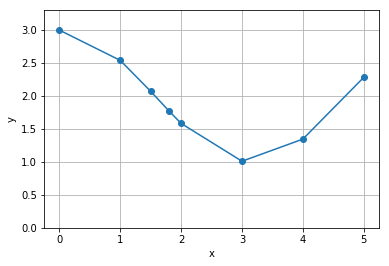
\includegraphics[width=\textwidth]{images/v9_integrate1}
\end{minipage}

\begin{minipage}[t]{0.49\textwidth}
	$\quad$\\[15pt]
	Integral (Fläche unter dem Graphen) berechnen:
\end{minipage}
\hspace{0.02\textwidth}
\begin{minipage}[t]{0.49\textwidth}
	\lstinputlisting{listings/v9_integrate3.py}
\end{minipage}


\pagebreak

\textbf{Gegebene Funktion}
\lstinputlisting{listings/v9_integrate4.py}

\section{Matplotlib}
\begin{itemize}
%	\item Tipps und Tricks in Jupyter
	\item Figure mit Subplots erstellen
	\item \texttt{plt.contour()} und \texttt{plt.contourf()}
	\item \texttt{plt.loglog()}
\end{itemize}

%\subsection{Tipps für Jupyter-Notebook}
%Folgende Zeile einfügen, damit man nicht immer \texttt{plt.show()} aufrufen muss
%\lstinputlisting{listings/v9_matplotlib1.py}
%Ein Semikolon am Zeilenende unterdrückt lästige Meldungen (\texttt{plt.plot(...);})

\subsection{Subplots}
\begin{minipage}[t]{0.49\textwidth}
	Einzelne Subplots nacheinander erstellen:
	\lstinputlisting{listings/v9_matplotlib2.py}
\end{minipage}
\hspace{0.02\textwidth}
\begin{minipage}[t]{0.49\textwidth}
	Alle Subplots von Anfang an erstellen:
	\lstinputlisting{listings/v9_matplotlib3.py}
	
\end{minipage}


\begin{minipage}[t]{0.49\textwidth}
	\subsection{Pyplot-Funktionen}
	\subsubsection{Treppensignal}
	\lstinputlisting{listings/v9_matplotlib4.py}
\end{minipage}
\hspace{0.02\textwidth}
\begin{minipage}[t]{0.49\textwidth}
	$\quad$\\[1pt]
	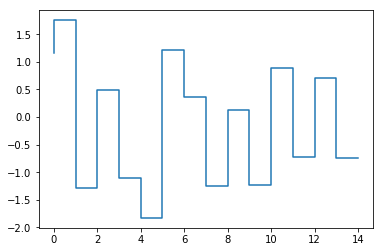
\includegraphics[width=0.8\textwidth]{images/v9_matplotlib1}
\end{minipage}

	\subsubsection{\texttt{contourf()}}
\url{https://matplotlib.org/api/_as_gen/matplotlib.pyplot.contourf.html}\\
\url{https://matplotlib.org/tutorials/colors/colormaps.html}\\
\begin{minipage}[t]{0.54\textwidth}
	\lstinputlisting{listings/v9_matplotlib5.py}
\end{minipage}
\hspace{0.02\textwidth}
\begin{minipage}[t]{0.44\textwidth}
	$\quad$\\[1pt]
	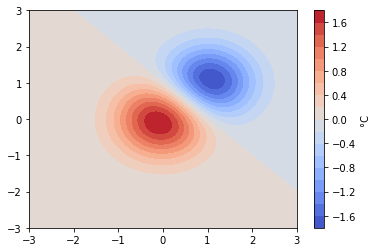
\includegraphics[width=0.9\textwidth]{images/v9_matplotlib2}
\end{minipage}




\subsubsection{\texttt{contour()}}
\url{https://matplotlib.org/api/_as_gen/matplotlib.pyplot.contour.html}\\
\begin{minipage}[t]{0.49\textwidth}
	\lstinputlisting{listings/v9_matplotlib6.py}
\end{minipage}
\hspace{0.02\textwidth}
\begin{minipage}[t]{0.49\textwidth}
	$\quad$\\[1pt]
	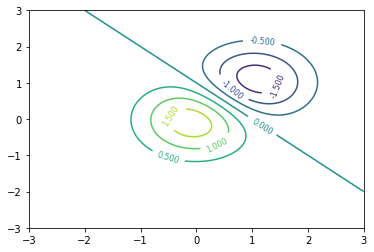
\includegraphics[width=0.75\textwidth]{images/v9_matplotlib3}
\end{minipage}


\subsubsection{\texttt{loglog()}}
\url{https://matplotlib.org/api/_as_gen/matplotlib.pyplot.loglog.html}\\
\begin{minipage}[t]{0.49\textwidth}
	\lstinputlisting{listings/v9_matplotlib7.py}
\end{minipage}
\hspace{0.02\textwidth}
\begin{minipage}[t]{0.49\textwidth}
	$\quad$\\[1pt]
	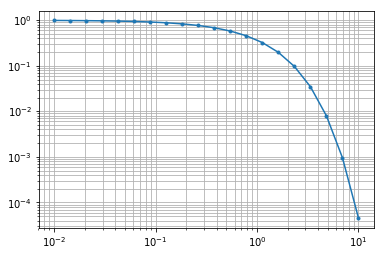
\includegraphics[width=0.75\textwidth]{images/v9_matplotlib4}
\end{minipage}




\subsubsection{XKCD}
\url{https://xkcd.com/}\\
\url{https://matplotlib.org/api/_as_gen/matplotlib.pyplot.xkcd.html}\\
\url{https://packages.debian.org/buster/fonts-humor-sans}\\
\url{https://github.com/shreyankg/xkcd-desktop/blob/master/Humor-Sans.ttf}\\
\begin{minipage}[t]{0.49\textwidth}
	\lstinputlisting{listings/v9_matplotlib8.py}
\end{minipage}
\hspace{0.02\textwidth}
\begin{minipage}[t]{0.49\textwidth}
	$\quad$\\[1pt]
	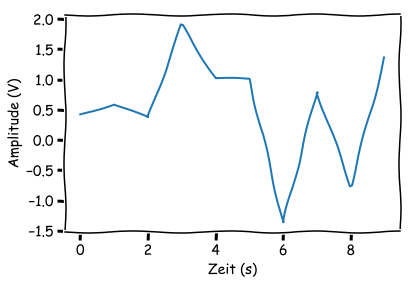
\includegraphics[width=0.75\textwidth]{images/v9_matplotlib5}
\end{minipage}

